\documentclass[aspectratio=169]{beamer}
\usetheme{Madrid}



\title{Basic Concepts in Machine Learning}
\author{Your Name}
\date{\today}

\begin{document}

\frame{\titlepage}

%------------------------------------------------
\begin{frame}{AI, ML, and Data Science Overlap}
\begin{figure}
    \centering
    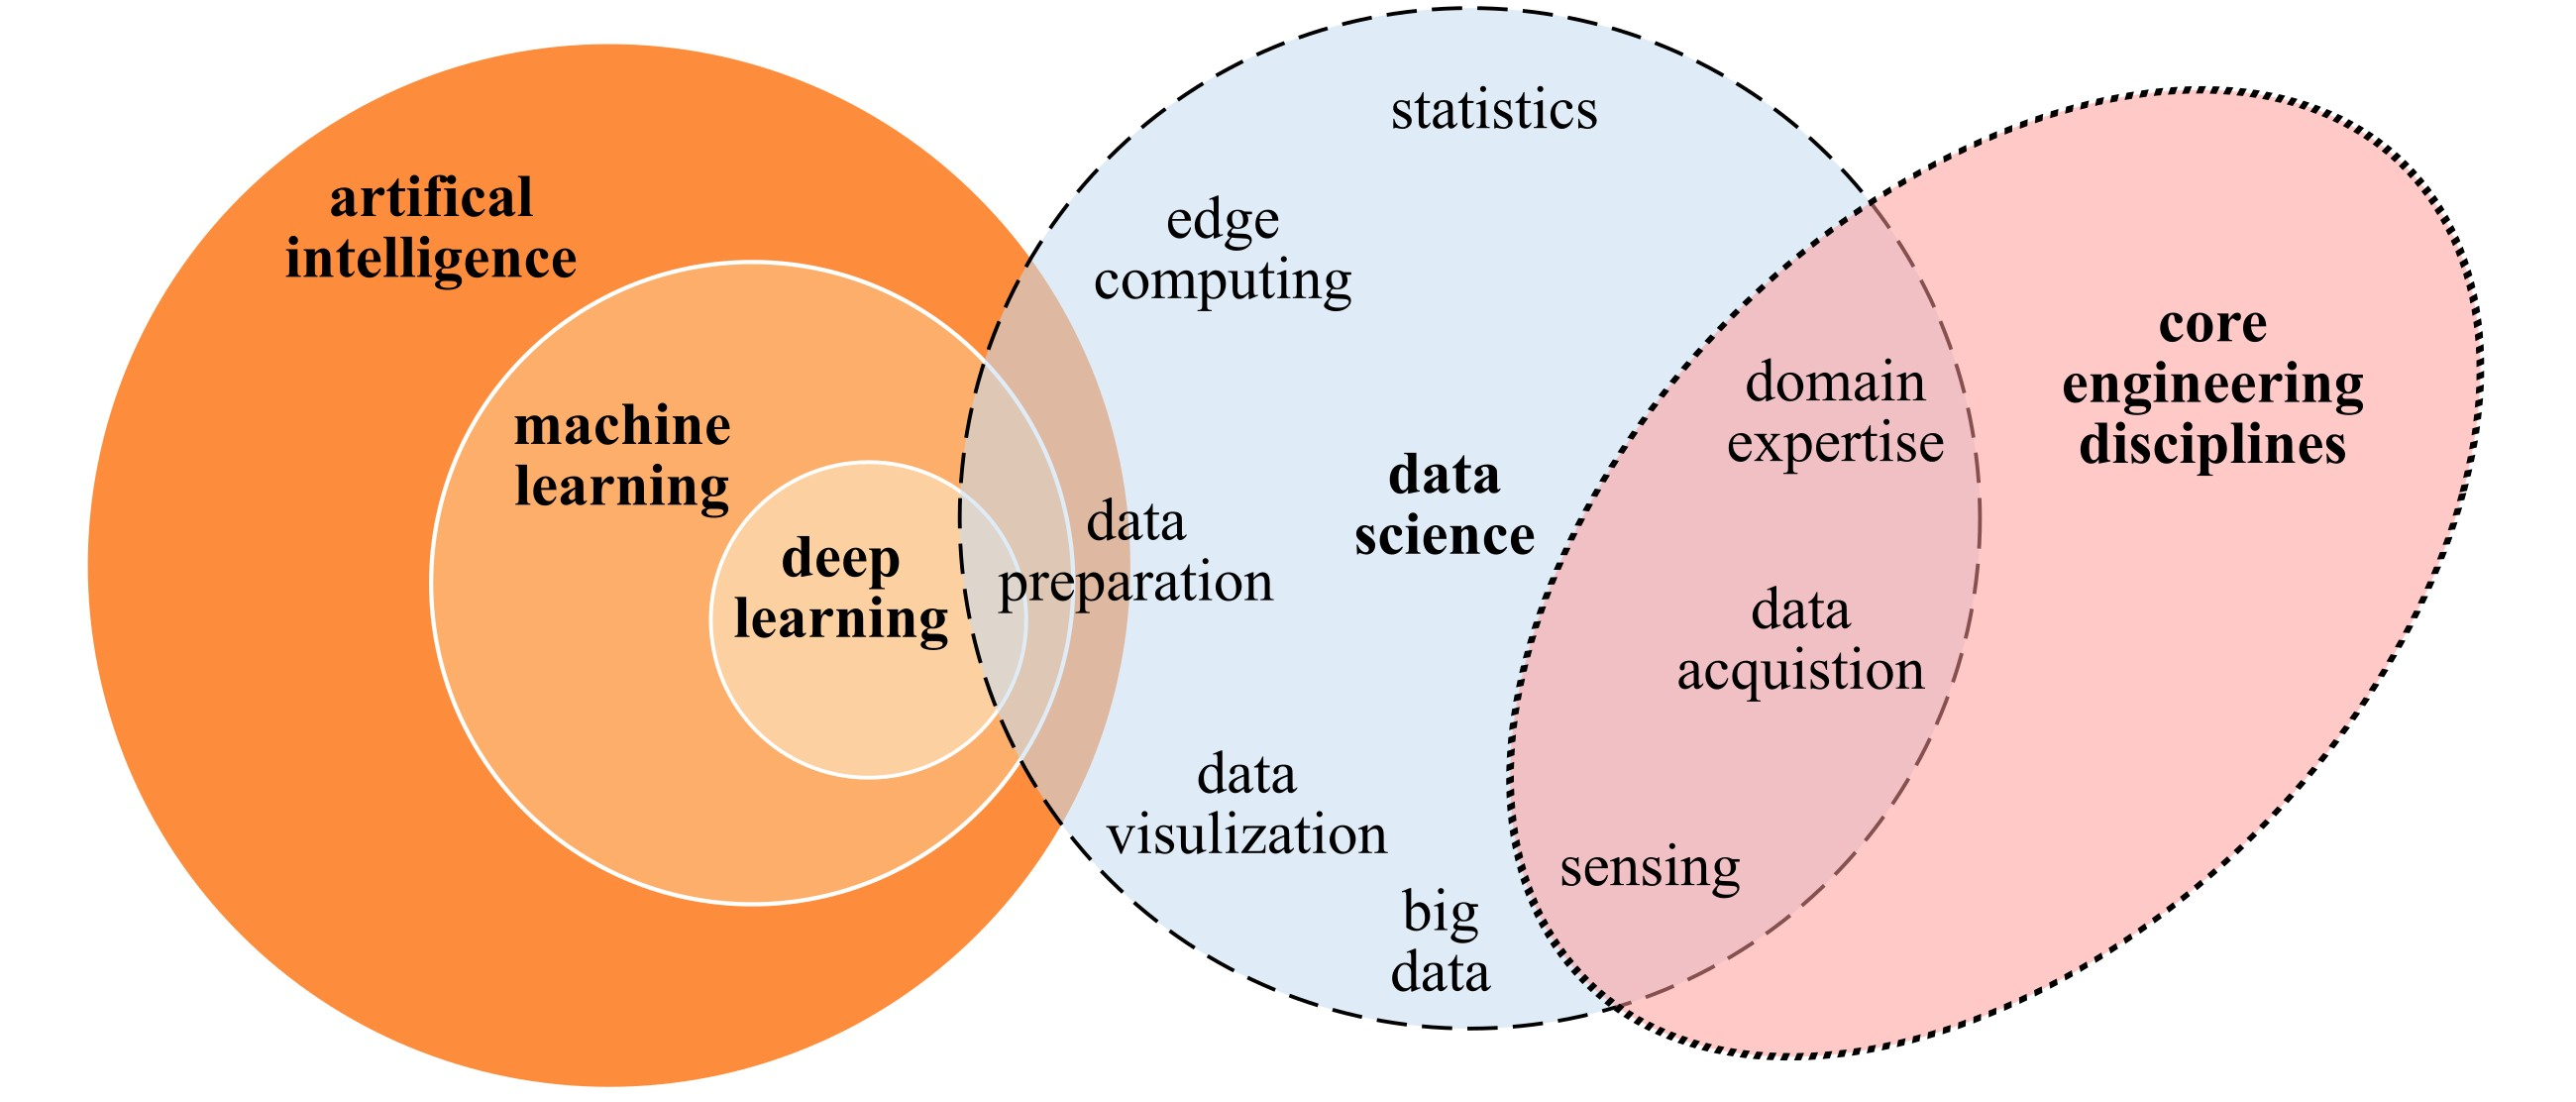
\includegraphics[width=\linewidth]{../figures/AI-vs-ML-vs-Deep-Learning}
    \caption{Overlap between AI, Data Science, and core engineering disciplines.}
\end{figure}
\end{frame}

%------------------------------------------------
\begin{frame}{What is Machine Learning?}
\begin{itemize}
    \item ML automates analytical model building.
    \item Closely tied to data science ? extracting insights from structured and unstructured data.
    \item Systems learn from data, identify patterns, and make decisions with minimal human intervention.
\end{itemize}
\end{frame}

%------------------------------------------------
\begin{frame}{Misconception: ML is Not About Robots}
\begin{itemize}
    \item ML is often confused with robotics.
    \item In reality, it focuses on algorithms that learn from data.
    \item Primary goal: prediction and decision-making from patterns in data.
\end{itemize}
\end{frame}

%------------------------------------------------
\begin{frame}{Early ML Applications}
\begin{itemize}
    \item \textbf{Spam filters} ? one of the first practical ML applications.
    \item \textbf{Speech-to-text} ? converting spoken language to written form.
    \item \textbf{Medical diagnostics} ? predicting diseases from medical data and images.
\end{itemize}
\end{frame}

%------------------------------------------------
\begin{frame}{Key ML Concepts \& Terminologies}
\begin{itemize}
    \item \textbf{Supervised vs Unsupervised Learning}  
    Train on labeled vs. unlabeled data.
    \item \textbf{Online vs Batch Learning}  
    Incremental updates vs. training all at once.
    \item \textbf{Instance-based vs Model-based Learning}  
    Memory-based predictions vs. generalized models.
\end{itemize}
\end{frame}

%------------------------------------------------
\begin{frame}{Expert Systems in AI}
\begin{figure}
    \centering
    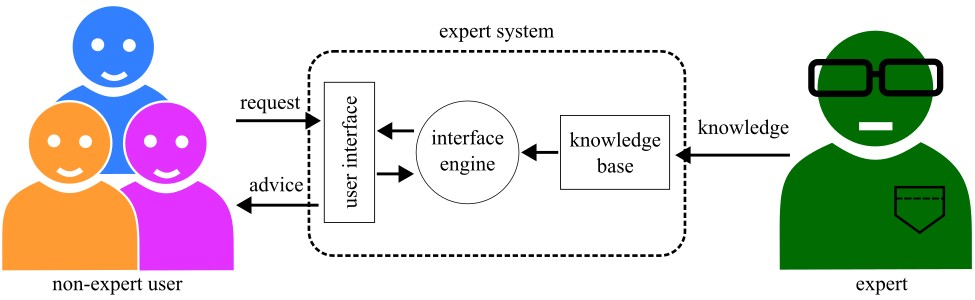
\includegraphics[width=0.9\linewidth]{../figures/expert_system}
    \caption{Expert systems simulate human decision-making using a knowledge base and inference rules.}
\end{figure}
\end{frame}

\begin{frame}{AI, ML, and Data Science Overlap}
\begin{itemize}
    \item AI is the broader field, ML is a subset, and Deep Learning is a subset of ML.
    \item Data Science intersects with all these domains.
\end{itemize}

\vspace{0.3cm}
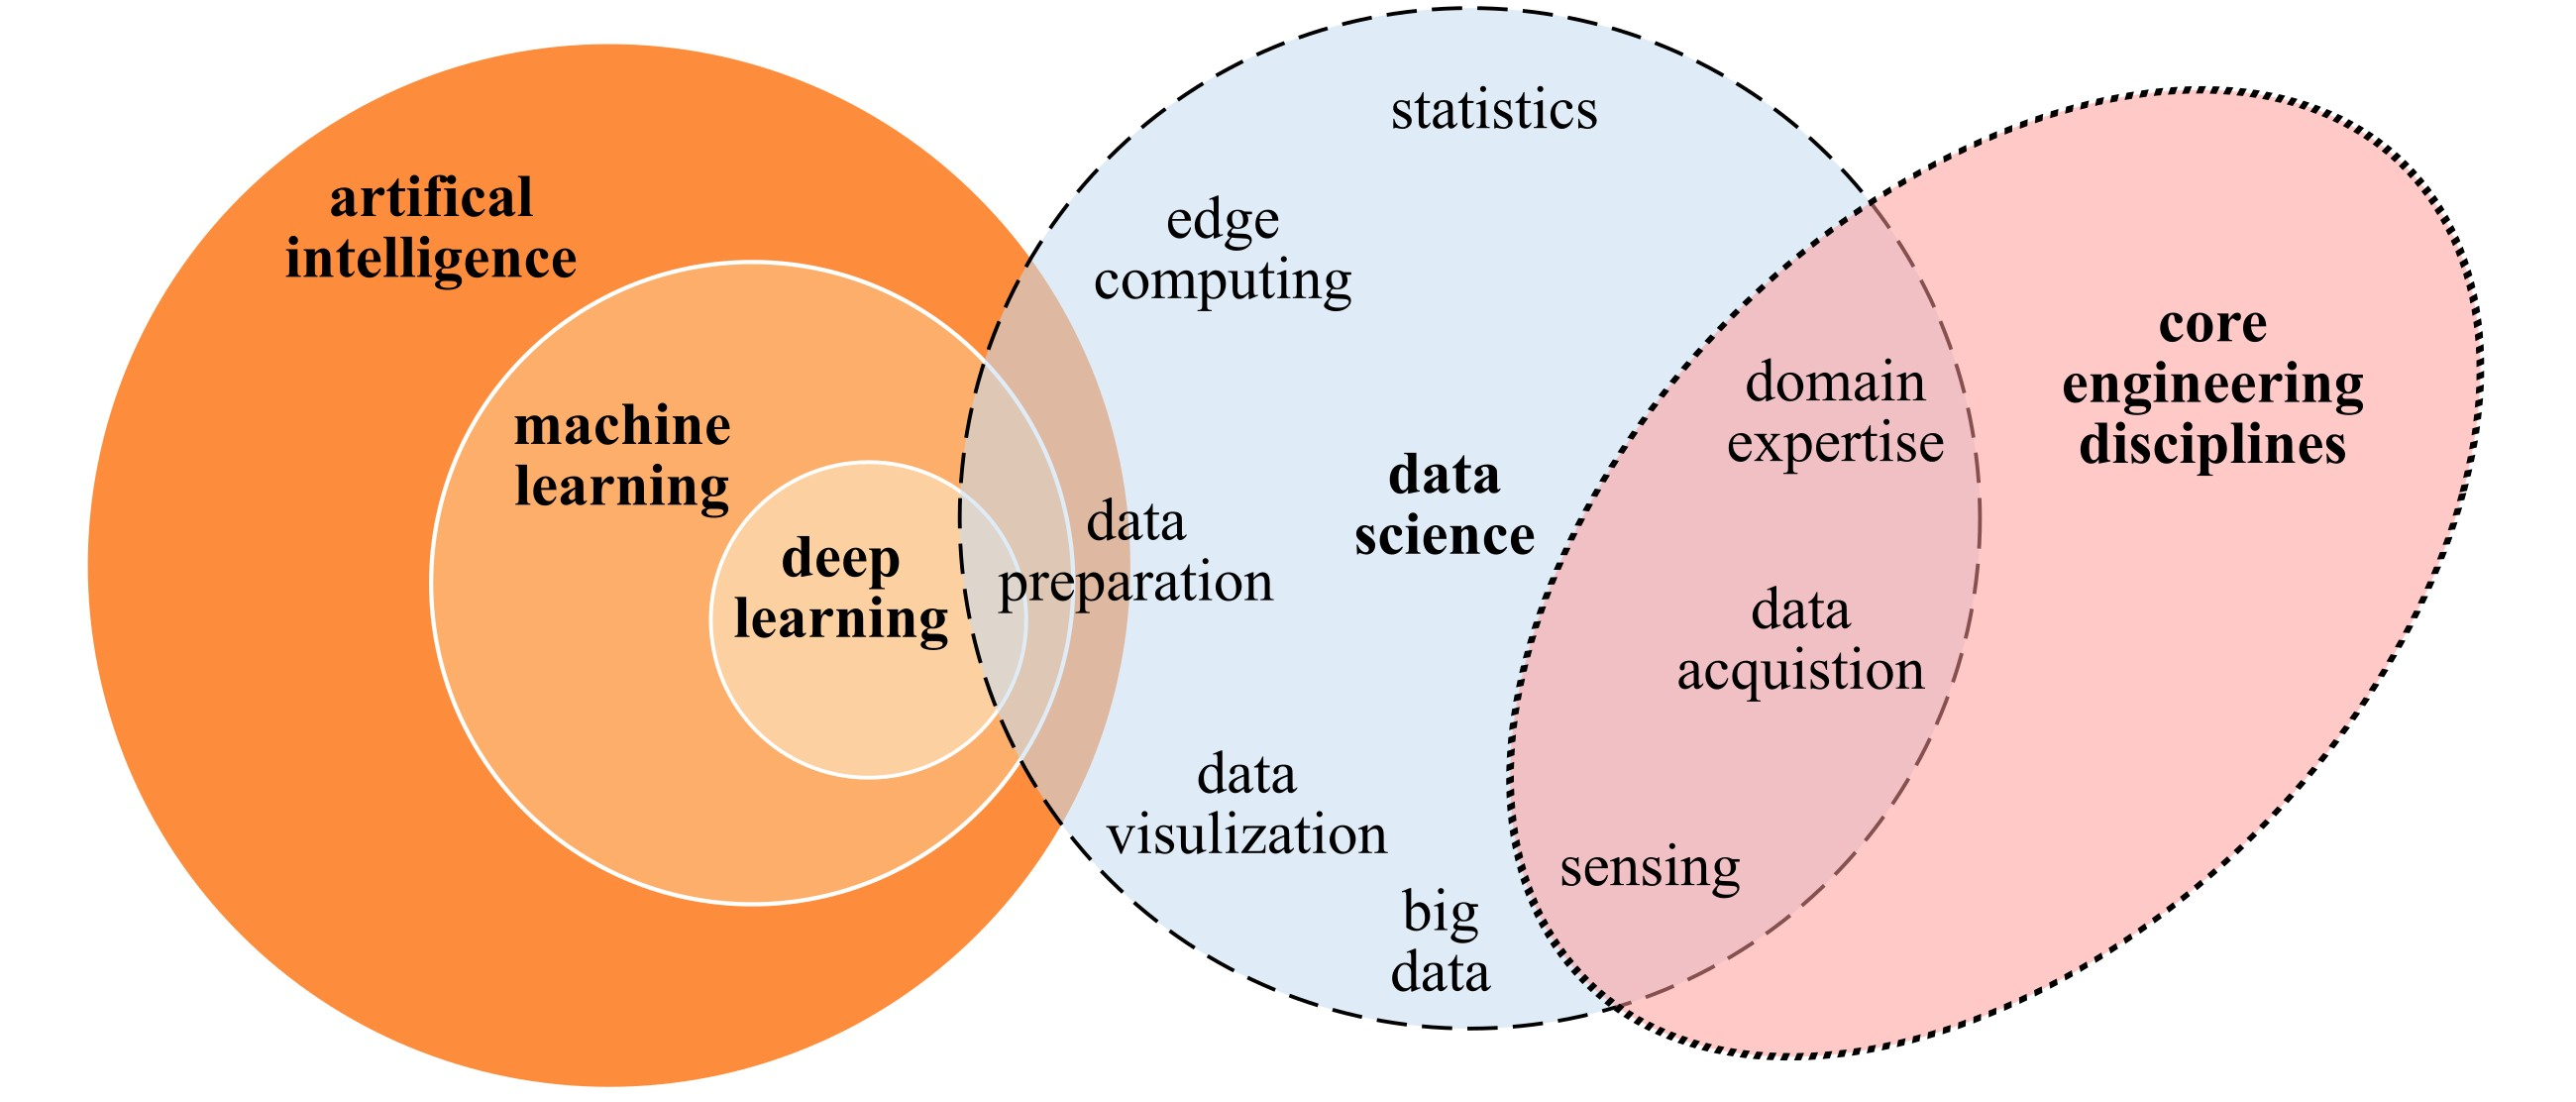
\includegraphics[width=\linewidth]{../figures/AI-vs-ML-vs-Deep-Learning}
\end{frame}

\end{document}




